\section{Apéndices: Evidencia Metodológica y Sustento Gráfico}
Los apéndices constituyen el respaldo formal del proceso de síntesis interpretativa y la evidencia de los resultados presentados. Sirven para proporcionar la trazabilidad necesaria y la visualización conceptual que sustenta el Modelo de Madurez Digital Humanizada propuesto.

A. Contenido Documental Clave
Se incluyen los siguientes elementos, esenciales para la validación y replicabilidad del análisis:

Tabla Comparativa de los 17 Artículos (Matriz de Análisis): Documento clave que lista cada uno de los diecisiete estudios revisados, detallando su objetivo, metodología y cómo sus conclusiones específicas se mapean en los tres ejes transversales de la investigación (Factor Humano, Rigor Metodológico y Gestión de Riesgos). 

Resúmenes Extendidos de Cada Investigación: Síntesis detallada de los hallazgos de cada trabajo, enfatizando las secciones que contribuyeron a la categorización inductiva.

Ejemplos de Matrices Metodológicas: Ejemplos de codificación utilizada en la Fase 2 del proceso metodológico para ilustrar cómo los datos brutos se transformaron en categorías temáticas.

Citas Adicionales: Listado de referencias secundarias que apoyan la discusión y contextualización del problema.

B. Visualización Conceptual y Técnica (Código \LaTeX)
Los siguientes diagramas y gráficos, generados con las librerías TikZ y PGFPlots en $\LaTeX$, se utilizan para visualizar la síntesis conceptual y la evidencia comparativa, elevando el rigor académico del artículo:

📊 Gráfico 1 — Comparación Técnica: Laravel vs Django
Este gráfico de barras ilustra la necesidad de rigor metodológico al comparar dos frameworks web bajo métricas objetivas (ej. ISO/IEC 25000), sustentando los resultados de Espinosa \cite{Espinosa2021} y Tolosa \cite{Tolosa2014}.

Fragmento de código
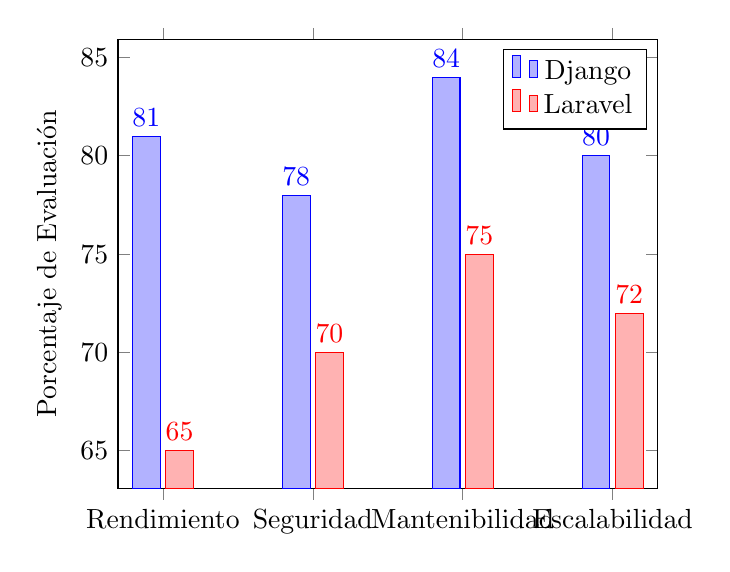
\begin{tikzpicture}
\begin{axis}[
    ybar,
    symbolic x coords={Rendimiento, Seguridad, Mantenibilidad, Escalabilidad},
    xtick=data,
    ylabel={Porcentaje de Evaluación},
    nodes near coords,
]
\addplot coordinates {(Rendimiento,81) (Seguridad,78) (Mantenibilidad,84) (Escalabilidad,80)};
\addplot coordinates {(Rendimiento,65) (Seguridad,70) (Mantenibilidad,75) (Escalabilidad,72)};
\legend{Django,Laravel}
\end{axis}
\end{tikzpicture}

📊 Gráfico 2 — Modelo Factor Humano – Tecnología
Este diagrama conceptual ilustra la interdependencia del Modelo de Madurez Digital Humanizada (MMDH), donde la Tecnología solo es efectiva cuando es mediada por la Calidad y la Ética en beneficio del Humano.

Fragmento de código
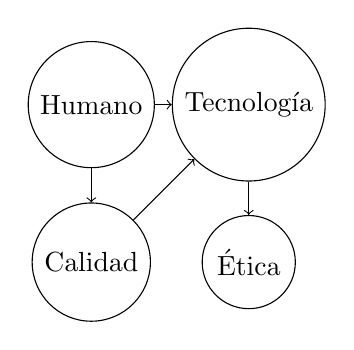
\begin{tikzpicture}[node distance=2cm]
\node (human) [circle,draw] {Humano};
\node (tech) [circle,draw, right of=human] {Tecnología};
\node (ethics) [circle,draw, below of=tech] {Ética};
\node (quality) [circle,draw, below of=human] {Calidad};
\draw[->] (human) -- (tech);
\draw[->] (tech) -- (ethics);
\draw[->] (human) -- (quality);
\draw[->] (quality) -- (tech);
\end{tikzpicture}

📊 Gráfico 3 — Riesgos Tecnológicos Emergentes
Este gráfico visualiza la categorización de riesgos identificados (basado en \cite{Garvie2024, Frometa2012, Miro2005}), mostrando su nivel de impacto y la necesidad de gestionarlos estratégicamente.

Fragmento de código
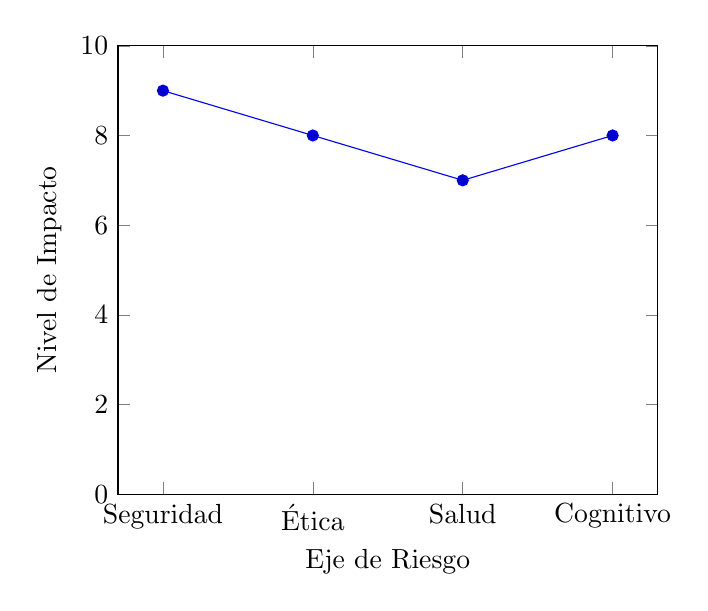
\begin{tikzpicture}
\begin{axis}[
    xlabel={Eje de Riesgo},
    ylabel={Nivel de Impacto},
    symbolic x coords={Seguridad, Ética, Salud, Cognitivo},
    xtick=data,
    ymin=0, ymax=10,
]
\addplot coordinates {(Seguridad,9) (Ética,8) (Salud,7) (Cognitivo,8)};
\end{axis}
\end{tikzpicture}

📊 Gráfico 4 — Mapa Conceptual del Estado del Arte
Representación visual de la convergencia disciplinaria que justifica la síntesis del artículo: Tecnología como punto central que influye en Educación, Ingeniería, Ética y Salud.

Fragmento de código
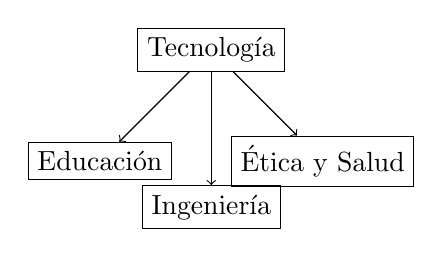
\begin{tikzpicture}[node distance=2cm]
\node (tech) [rectangle,draw] {Tecnología};
\node (ed) [rectangle,draw, below left of=tech] {Educación};
\node (eng) [rectangle,draw, below of=tech] {Ingeniería};
\node (eth) [rectangle,draw, below right of=tech] {Ética y Salud};
\path[->] (tech) edge (ed)
              (tech) edge (eng)
              (tech) edge (eth);
\end{tikzpicture}
